\section{Implementation}

\subsection{Build plan}

\blindtext

\subsection{Prototyping}

\subsubsection{DAW: Static}

Our DAW prototype was constructed without the use of the Electron UI-building environment. This
decision was motivated by the belief that creating the Electron application encompassed two
separate problems: the first was to create a fully functioning script, the second was to port that
script into the Electron application. By building the prototype outside of Electron, we aimed for
faster progress and less bottlenecking of the workflow by dealing with one smaller problem at a
time. Additionally, this decision expedited the debugging process by removing the need to load
the full Electron application every time we wished to monitor the progress of the build. Instead,
we could simply locate the HTML file in out directory and open it in a browser with a single click.

The first step in constructing the DAW was to establish all of the static elements, which include
the piano roll (which is displayed inside a horizontally-scrolling container), the guide keys, and
the menu buttons.

The \textbf{piano roll} is the space in which the user can design their MIDI by adding,
moving, and removing notes. It appears as a rectangular space adorned with horizontal stripes. Each
white stripe corresponds to the vertical position that represents a white key on the keyboard, and
the same goes for the black stripes corresponding to black keys. Progressing upward in the pattern
of stripes is equivalent to progressing left to right on the keyboard. The guide keys follow a
similar format to the piano roll, with black and white stripes that visualize a piano keyboard
rotated 90 degrees counter-clockwise. Unlike the piano roll, however, the guide keys are much
shorter in width and remain as a static element outside (to the left) of the scroll container.
The stripes also display the name of the note to which they correspond. This allows the guide keys
to act as a reference for the user, so they can easily see which note each piano roll stripe
represents without having to count from the bottom. To serve this purpose properly, it is
imperative that the guide keys' stripes line up exactly with those on the piano roll.

This was achieved by building both assets using the same grid display class, given the name
"piano-container." In the CSS script, the piano-container class was styled as a grid display,
which established the appropriate pattern of black and white key items and set a standard gap of
one pixel between each key. The key items were then added as rectangular DIV objects with the
appropriate background color and a standard height of ten pixels. The guide keys were assigned an
additional class called "keys," which gave them a set width. Text was added in the center of each
DIV, labelling it by note. The piano roll was assigned the additional class "roll," which lowered
the opacity of the stripes to allow for better readability. The roll class also gave the piano roll
the absolute position attribute which allowed it to scroll within the scroll container.

At this stage of development, the dimensions of the screen upon which the DAW was to be displayed
were unknown. To proceed with prototyping at a timely pace, we made the width of the piano roll
flexible by reading the size of the window upon opening and setting the piano roll's width
attribute relative to the result. This means that the dimensions may not function properly if the
window is resized after opening, but this is not expected to be a problem because there will be
no way for the user to change the window size on the final keyboard.

The \textbf{menu buttons} were added below the scroll container, separated into one group which is flush
left, and another which is flush right. The left button group deals with the state of the piano
roll; these buttons allow the user save the state, reset it to its last save, and utilize undo and
redo functions to return the piano roll to a previous state. There is also a tempo button which
allows the user to select the tempo of playback. The right button group deals with the mode of
interaction. Depending on which of these buttons is selected, the users will be able to switch
between adding, deleting, moving, and stretching the notes on the roll. There are also play and
stop buttons that control playback, and a quantization button that can change the size and
positions the notes will snap to when editing. There is one additional button not included among
the menu buttons. This button exists on the far right of the piano roll, labelled with a plus sign.
It allows users to extend the piano roll so that they may create a longer melody.

\begin{figure}[h!]
  \centering
  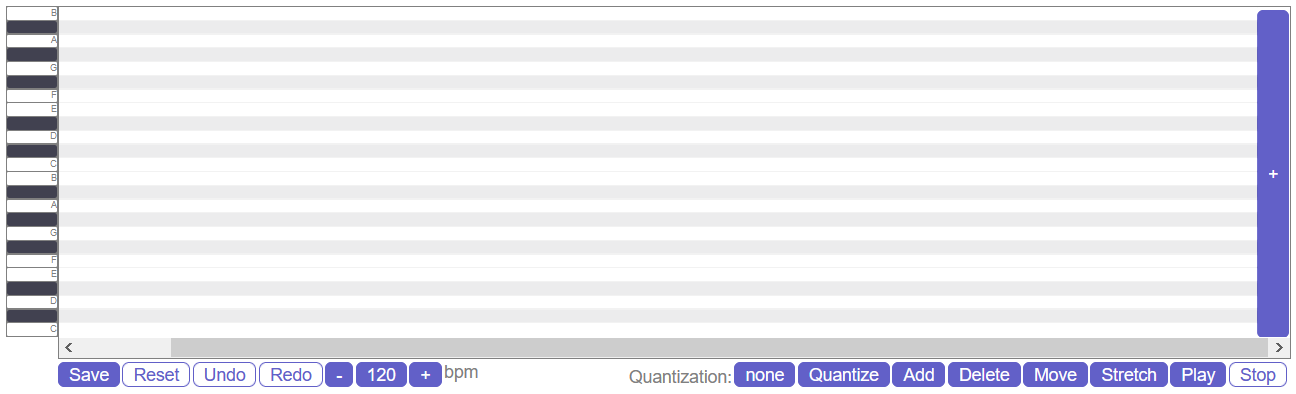
\includegraphics[width=\linewidth]{image/Static.png}
  \caption{A snapshot of the static assets of the DAW, the piano roll is empty}
  \label{fig:static}
\end{figure}

All UI buttons belong to the CSS class "ui," which gives them a uniform design. This class adds
several cosmetic elements to enhance the user experience by making interactions more visually
pleasing. The buttons have a periwinkle color and rounded corners to make them feel softer and
more polished than the default HTML button. They also expand in size and invert in color when
moused over to indicate they can be clicked. To make this transformation feel fluid, the transition
time has been set to 0.4 seconds, as opposed to the default 0 seconds which would have the buttons
snap immediately from one state to the next. Buttons that are disabled and cannot be clicked are
displayed at the standard size but with inverted colors.

\begin{figure}[h!]
  \centering
  
\includegraphics{image/StdUI.png}
  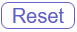
\includegraphics{image/HoverUI.png}
  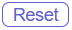
\includegraphics{image/DisabledUI.png}
  \caption{A sample of the styling of the menu buttons in their standard, hover, and disabled states respectively}
  \label{fig:ui_variations}
\end{figure}

UI buttons are enabled and disabled on a situational basis to prevent the user from interacting
with the application in an unintended manner. For example, The "Undo" button is disabled if no
edits have been made to the notes or if the user has reverted state using this button more than
the allotted number of times with no edits between. This prevents the user from reverting state
farther back than the original state upon opening. Similarly, the "Redo" button is disabled until
the "Undo" button has been pressed and disables again when any edits are made to the notes. This
prevents the users from redoing an undone state after an edit has been made, thus overwriting any
edits made since the "Undo" button was used. The "Reset" button is disabled only when the program
has just been opened or reset and no edits to the notes have been made since. This is not so much
to prevent the user from pressing it again, but more so to indicate to the user that resetting the
state again would be unnecessary and redundant. The "Play" button is only disabled when
the MIDI playback is active, while the "Stop" button behaves oppositely. Much like the "Reset"
button, this is primarily designed to indicate redundancy in an interaction, but also if the "Play"
button were to be pressed during MIDI playback, a second audio instance of the MIDI would begin
playing over top of the first. Finally, each of the mode buttons (Add, Delete, Move, and Stretch)
is disabled when its mode is active, to indicate to the user which edit mode the application is
currently running.

The \textbf{MIDI notes} have been implemented in the form of buttons. These buttons have their own CSS
class, appropriately named "note," that give them a polished uniform look. For cohesion, the note
border is the same color as the buttons and the fill color is a slightly lighter shade. They also
have rounded corners to maintain the same polished feel as the menu buttons. The fill color
lightens when the note is hovered over to indicate to the user which element they are selecting.
This transformation could not be given a transition time like the menu buttons, though, because
extending the transition time would also extend the time the note takes to move around when being
dragged by the user.

The prototype opens with the first two lines of \textit{Twinkle, Twinkle, Little Star} as the default
melody. For each note, the program determines the position and dimensions based on its attributes
in the MIDI file. The heights of the notes are set equal to the height of the key template on the
piano roll so that they may align perfectly on top of the piano roll stripes. The vertical position
is assigned based on the note's pitch. MIDI pitch values start at 0 representing C in the -1 octave
and each integer increase represents an ascent of one diatonic step in the key of C. Our keyboard
prototype spans two octaves, with Middle C (C in the 4th octave) at its lowest extreme, so it
handles pitch values 60-83. To translate these pitch values into a vertical position, we
implemented the following formula:

\begin{equation} \label{note_vert}
top_{note} = \Big((height_{note} + key\:gap) * 23 - \big((pitch_{note} -  60) * (height_{note} + key\:gap)\big)\Big)\:pixels
\end{equation}

Because the vertical position is measured in the number of pixels between the top of the parent
window and the top of the element, the first section of this formula $ (height_{note} + keygap) * 23 $
establishes that the search for the vertical position is based 23 keys from the top, which is
the lowest key on a two-octave keyboard. The second section $ (pitch_{note} -  60) * (height_{note} + keygap)) $
shows that the base pitch is 60, and that the note's height above the the base key will be
proportional to the difference between the note's pitch and the base pitch in units equal to the
key height (maintaining the key gap in between).

The horizontal position is assigned based on the note's start time and the playback tempo. The
start time attribute in MIDI data is measured in seconds. Our prototype represents a whole note
with a width of 64 pixels, so the horizontal position of the note is determined by the following
formula:

\begin{equation} \label{note_vert}
left_{note} = \frac{start\:time * 60}{tempo} * 64\:pixels
\end{equation}

The multiplication of the start time by 60 and subsequent division by the playback tempo
establishes the ratio between one second and one whole note. So through this, the number of
seconds is translated into a number of whole notes, and the final multiplication by 64 - the width
of a whole note - places the note at the corresponding beat on the piano roll.

The width of the note is similarly calculated based on the start time, end time, and tempo:

\begin{equation} \label{note_vert}
width_{note} = \frac{(end\:time - start\:time) * 60}{tempo} * 64\:pixels
\end{equation}

The difference between the start and end time is converted to some decimal number of whole note
lengths, and this is translated into the width of the note in pixels.

\subsubsection{DAW: Functional}

Once the visual layout of the DAW had been established, we added interactivity in JavaScript. The
first function implemented was editing the note sequence by moving the notes, because this is
arguably the most used and therefore most important feature of a DAW. At this phase of development,
the methods of input were yet unknown - we intended to either use a single-touch touch screen or a
cursor controlled by arrow keys. The important thing to consider about how this affects UI design
is that moving an element in a 2D space requires a decent degree of freedom in the user inputs.
Single-touch touchscreens and arrow key cursors both provide limited input, but each lending to a
different style of interaction. To account for both possibilities, two versions of the note moving
function were developed: a click-and-drag version suited for touchscreen input and a click-to-
select/click-again-to-place version suited for arrow key input.

Rather than being on-click functions for the notes, each edit function is called with the notes as
its argument once the DAW has entered the corresponding edit mode. This is because the on-click
function of the notes must be edited at different points of interaction within the edit mode. At
its start, the click-and-drag move function sets the notes' on-mouse-down function to change the
on-mouse-move and on-mouse-up function. This means that the notes will not respond to cursor
movements unless the cursor has clicked and is holding over the note. The on-mouse-up function
resets the on-mouse-move and on-mouse-up functions to null, so once the mouse is released, the note
no longer responds to mouse movement. The activated on-mouse-move function will continuously edit
the position attributes of the note so that the note follows the cursor while snapping to valid
positions as determined by the quantization and available pitches.

\subsection{Testing}

\blindtext

\subsection{Evaluation}

\blindtext
